\textbf{Problem}: How to build ChatGPT?

\textbf{Assumption}: Producing \& Understanding language are strongly related: If a model can predict how a text continues, it must have understood \textit{something} about language \& meaning.

\definition \textbf{Language Model}: A prob. distrib. over words/sentences

The model should assign high prob. to \textit{plausible} texts: 
$$
    \P\bigl[\text{"I like to eat pasta"}\bigr] > \P\bigl[\text{"I rocks like eat to"}\bigr]
$$

A simple model, exponential in $m$, would be:
$$
    P\bigl( \underbrace{\text{Sentence}}_\text{Length $m$} \bigr) = P\Bigl(\underbrace{X_1=x_1}_\text{1st word}, \underbrace{X_2=x_2}_\text{2nd word},\ldots,X_m=x_m \Bigr)
$$

{\footnotesize
    \remark In practice, \textit{Tokens} are used instead of words. Tokens are "units of meaning" obtained from a sentence, e.g. seperating "don't" into "do" and "n't", to improve processing.
}

\subsection{Autoregressive models}

\textbf{Idea}: Abuse the chain rule of probability.
$$
    P(x_1,x_2,\ldots,x_m) = P(x_1)P(x_2|x_2)\cdots P(x_m|x_1,\ldots,x_{m-1})
$$
This lends itself very naturally to sentence generation:
\begin{align*}
    x_1 \sim P(X_1) \quad x_2 \sim P(X_2\sep X_1=x_1) \quad \ldots
\end{align*}
Essentially: Sample a token (next word) from the cond. distrib. (sentence so far) at each step. This avoids computing the entire joint distribution.

{\footnotesize
    \remark Model outputs are inputs for next prediction: \textit{Autoregressive}.
}

\begin{center}
    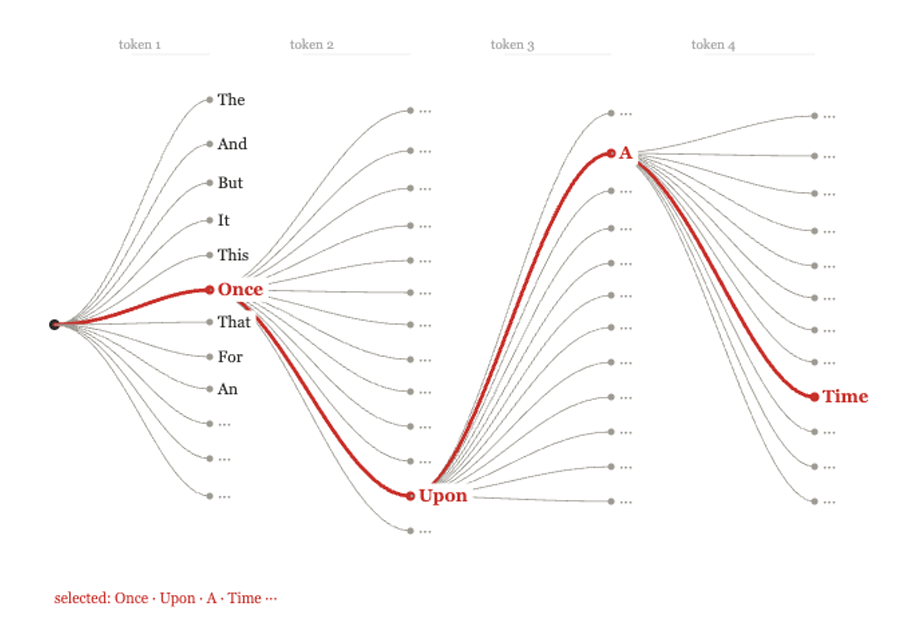
\includegraphics[width=0.6\linewidth]{resources/Autoregressor.png}\\
    \footnotesize\color{gray}\textit{Introduction to Machine Learning (2026), p. 277}
\end{center}

\subsubsection{Neural Network Language Models}

Instead of looking at all previous words, only the recent $k$:\\
\subtext{This is called \textit{Context length}}
\begin{align*}
            &P\bigl( X_t=x\sep X_{1:t-1} = x_{1:t-1} \bigr)                                     \\
    \approx &P\bigl(X_t=x\sep X_{t-k:t-1} = x_{t-k:t-1}, \theta\bigr)                           \\
    :=      & \text{Cat}\bigl( x \sep \text{softmax}\bigl( f(x_{t-k:t-1}, \theta) \bigr) \bigr)
\end{align*}

\textbf{Optimization Problem}:
$$
    \underset{\theta}{\min} L(\theta) := \underbrace{-\sum_{t}\log\Bigl( P\bigl( X_t=x_t\sep X_{t-k:t-1} = x_{t-k:t-1}, \theta \bigr) \Bigr)}_\text{Negative Log-Likelihood}  
$$

This is a form of \textit{Self-Supervision}: No labels are needed.\\
In Datasets, the next word $x_t$ is the prediction target.\\
\subtext{Thus: \textit{Any text} can be used as a training set}

\subsubsection{Input Representation}

Preparing inputs roughly follows this idea:
$$
    \text{Language} \underset{\text{Tokenization}}{\mapsto} \text{Tokens} \underset{\text{Vectorization}}{\mapsto} \text{Vector}
$$

\definition \textbf{Word Embedding Matrix} $\quad \mathbf{W}_e \in \R^{N\times d}, d \ll N$\\ 
\subtext{$N$ is the vocabulary size}

Each token receives a position in $d$-dimensional space: Semantically similar tokens are closer.

{\footnotesize
    \remark \textbf{One-Hot Encoding}\\
    Bad for many reasons: dimension $\propto$ vocabulary size, dot product is always zero (every input equally "dissimilar")
}

\newpage
\subsection{Transformers \& Attention}

